%% bare_jrnl.tex
%% V1.4b
%% 2015/08/26
%% by Michael Shell
%% see http://www.michaelshell.org/
%% for current contact information.
%%
%% This is a skeleton file demonstrating the use of IEEEtran.cls
%% (requires IEEEtran.cls version 1.8b or later) with an IEEE
%% journal paper.
%%
%% Support sites:
%% http://www.michaelshell.org/tex/ieeetran/
%% http://www.ctan.org/pkg/ieeetran
%% and
%% http://www.ieee.org/

%%*************************************************************************
%% Legal Notice:
%% This code is offered as-is without any warranty either expressed or
%% implied; without even the implied warranty of MERCHANTABILITY or
%% FITNESS FOR A PARTICULAR PURPOSE! 
%% User assumes all risk.
%% In no event shall the IEEE or any contributor to this code be liable for
%% any damages or losses, including, but not limited to, incidental,
%% consequential, or any other damages, resulting from the use or misuse
%% of any information contained here.
%%
%% All comments are the opinions of their respective authors and are not
%% necessarily endorsed by the IEEE.
%%
%% This work is distributed under the LaTeX Project Public License (LPPL)
%% ( http://www.latex-project.org/ ) version 1.3, and may be freely used,
%% distributed and modified. A copy of the LPPL, version 1.3, is included
%% in the base LaTeX documentation of all distributions of LaTeX released
%% 2003/12/01 or later.
%% Retain all contribution notices and credits.
%% ** Modified files should be clearly indicated as such, including  **
%% ** renaming them and changing author support contact information. **
%%*************************************************************************


% *** Authors should verify (and, if needed, correct) their LaTeX system  ***
% *** with the testflow diagnostic prior to trusting their LaTeX platform ***
% *** with production work. The IEEE's font choices and paper sizes can   ***
% *** trigger bugs that do not appear when using other class files.       ***                          ***
% The testflow support page is at:
% http://www.michaelshell.org/tex/testflow/


% Please refer to your journal's instructions for other
% options that should be set.
\documentclass[journal,onecolumn]{IEEEtran}
%
% If IEEEtran.cls has not been installed into the LaTeX system files,
% manually specify the path to it like:
% \documentclass[journal]{../sty/IEEEtran}





% Some very useful LaTeX packages include:
% (uncomment the ones you want to load)


% *** MISC UTILITY PACKAGES ***
%
%\usepackage{ifpdf}
% Heiko Oberdiek's ifpdf.sty is very useful if you need conditional
% compilation based on whether the output is pdf or dvi.
% usage:
% \ifpdf
%   % pdf code
% \else
%   % dvi code
% \fi
% The latest version of ifpdf.sty can be obtained from:
% http://www.ctan.org/pkg/ifpdf
% Also, note that IEEEtran.cls V1.7 and later provides a builtin
% \ifCLASSINFOpdf conditional that works the same way.
% When switching from latex to pdflatex and vice-versa, the compiler may
% have to be run twice to clear warning/error messages.



\usepackage{caption}


% *** CITATION PACKAGES ***
%
\usepackage{cite}
% cite.sty was written by Donald Arseneau
% V1.6 and later of IEEEtran pre-defines the format of the cite.sty package
% \cite{} output to follow that of the IEEE. Loading the cite package will
% result in citation numbers being automatically sorted and properly
% "compressed/ranged". e.g., [1], [9], [2], [7], [5], [6] without using
% cite.sty will become [1], [2], [5]--[7], [9] using cite.sty. cite.sty's
% \cite will automatically add leading space, if needed. Use cite.sty's
% noadjust option (cite.sty V3.8 and later) if you want to turn this off
% such as if a citation ever needs to be enclosed in parenthesis.
% cite.sty is already installed on most LaTeX systems. Be sure and use
% version 5.0 (2009-03-20) and later if using hyperref.sty.
% The latest version can be obtained at:
% http://www.ctan.org/pkg/cite
% The documentation is contained in the cite.sty file itself.






% *** GRAPHICS RELATED PACKAGES ***
%
\ifCLASSINFOpdf
  \usepackage[pdftex]{graphicx}
  % declare the path(s) where your graphic files are
  \graphicspath{/figures}
  % and their extensions so you won't have to specify these with
  % every instance of \includegraphics
  \DeclareGraphicsExtensions{.pdf,.jpeg,.png}
\else
  % or other class option (dvipsone, dvipdf, if not using dvips). graphicx
  % will default to the driver specified in the system graphics.cfg if no
  % driver is specified.
  % \usepackage[dvips]{graphicx}
  % declare the path(s) where your graphic files are
  % \graphicspath{{../eps/}}
  % and their extensions so you won't have to specify these with
  % every instance of \includegraphics
  % \DeclareGraphicsExtensions{.eps}
\fi
% graphicx was written by David Carlisle and Sebastian Rahtz. It is
% required if you want graphics, photos, etc. graphicx.sty is already
% installed on most LaTeX systems. The latest version and documentation
% can be obtained at: 
% http://www.ctan.org/pkg/graphicx
% Another good source of documentation is "Using Imported Graphics in
% LaTeX2e" by Keith Reckdahl which can be found at:
% http://www.ctan.org/pkg/epslatex
%
% latex, and pdflatex in dvi mode, support graphics in encapsulated
% postscript (.eps) format. pdflatex in pdf mode supports graphics
% in .pdf, .jpeg, .png and .mps (metapost) formats. Users should ensure
% that all non-photo figures use a vector format (.eps, .pdf, .mps) and
% not a bitmapped formats (.jpeg, .png). The IEEE frowns on bitmapped formats
% which can result in "jaggedy"/blurry rendering of lines and letters as
% well as large increases in file sizes.
%
% You can find documentation about the pdfTeX application at:
% http://www.tug.org/applications/pdftex





% *** MATH PACKAGES ***
%
\usepackage{amsmath}
% A popular package from the American Mathematical Society that provides
% many useful and powerful commands for dealing with mathematics.
%
% Note that the amsmath package sets \interdisplaylinepenalty to 10000
% thus preventing page breaks from occurring within multiline equations. Use:
\interdisplaylinepenalty=2500
% after loading amsmath to restore such page breaks as IEEEtran.cls normally
% does. amsmath.sty is already installed on most LaTeX systems. The latest
% version and documentation can be obtained at:
% http://www.ctan.org/pkg/amsmath





% *** SPECIALIZED LIST PACKAGES ***
%
%\usepackage{algorithmic}
% algorithmic.sty was written by Peter Williams and Rogerio Brito.
% This package provides an algorithmic environment fo describing algorithms.
% You can use the algorithmic environment in-text or within a figure
% environment to provide for a floating algorithm. Do NOT use the algorithm
% floating environment provided by algorithm.sty (by the same authors) or
% algorithm2e.sty (by Christophe Fiorio) as the IEEE does not use dedicated
% algorithm float types and packages that provide these will not provide
% correct IEEE style captions. The latest version and documentation of
% algorithmic.sty can be obtained at:
% http://www.ctan.org/pkg/algorithms
% Also of interest may be the (relatively newer and more customizable)
% algorithmicx.sty package by Szasz Janos:
% http://www.ctan.org/pkg/algorithmicx




% *** ALIGNMENT PACKAGES ***
%
%\usepackage{array}
% Frank Mittelbach's and David Carlisle's array.sty patches and improves
% the standard LaTeX2e array and tabular environments to provide better
% appearance and additional user controls. As the default LaTeX2e table
% generation code is lacking to the point of almost being broken with
% respect to the quality of the end results, all users are strongly
% advised to use an enhanced (at the very least that provided by array.sty)
% set of table tools. array.sty is already installed on most systems. The
% latest version and documentation can be obtained at:
% http://www.ctan.org/pkg/array


% IEEEtran contains the IEEEeqnarray family of commands that can be used to
% generate multiline equations as well as matrices, tables, etc., of high
% quality.




% *** SUBFIGURE PACKAGES ***
%\ifCLASSOPTIONcompsoc
%  \usepackage[caption=false,font=normalsize,labelfont=sf,textfont=sf]{subfig}
%\else
%  \usepackage[caption=false,font=footnotesize]{subfig}
%\fi
% subfig.sty, written by Steven Douglas Cochran, is the modern replacement
% for subfigure.sty, the latter of which is no longer maintained and is
% incompatible with some LaTeX packages including fixltx2e. However,
% subfig.sty requires and automatically loads Axel Sommerfeldt's caption.sty
% which will override IEEEtran.cls' handling of captions and this will result
% in non-IEEE style figure/table captions. To prevent this problem, be sure
% and invoke subfig.sty's "caption=false" package option (available since
% subfig.sty version 1.3, 2005/06/28) as this is will preserve IEEEtran.cls
% handling of captions.
% Note that the Computer Society format requires a larger sans serif font
% than the serif footnote size font used in traditional IEEE formatting
% and thus the need to invoke different subfig.sty package options depending
% on whether compsoc mode has been enabled.
%
% The latest version and documentation of subfig.sty can be obtained at:
% http://www.ctan.org/pkg/subfig




% *** FLOAT PACKAGES ***
%
%\usepackage{fixltx2e}
% fixltx2e, the successor to the earlier fix2col.sty, was written by
% Frank Mittelbach and David Carlisle. This package corrects a few problems
% in the LaTeX2e kernel, the most notable of which is that in current
% LaTeX2e releases, the ordering of single and double column floats is not
% guaranteed to be preserved. Thus, an unpatched LaTeX2e can allow a
% single column figure to be placed prior to an earlier double column
% figure.
% Be aware that LaTeX2e kernels dated 2015 and later have fixltx2e.sty's
% corrections already built into the system in which case a warning will
% be issued if an attempt is made to load fixltx2e.sty as it is no longer
% needed.
% The latest version and documentation can be found at:
% http://www.ctan.org/pkg/fixltx2e


%\usepackage{stfloats}
% stfloats.sty was written by Sigitas Tolusis. This package gives LaTeX2e
% the ability to do double column floats at the bottom of the page as well
% as the top. (e.g., "\begin{figure*}[!b]" is not normally possible in
% LaTeX2e). It also provides a command:
%\fnbelowfloat
% to enable the placement of footnotes below bottom floats (the standard
% LaTeX2e kernel puts them above bottom floats). This is an invasive package
% which rewrites many portions of the LaTeX2e float routines. It may not work
% with other packages that modify the LaTeX2e float routines. The latest
% version and documentation can be obtained at:
% http://www.ctan.org/pkg/stfloats
% Do not use the stfloats baselinefloat ability as the IEEE does not allow
% \baselineskip to stretch. Authors submitting work to the IEEE should note
% that the IEEE rarely uses double column equations and that authors should try
% to avoid such use. Do not be tempted to use the cuted.sty or midfloat.sty
% packages (also by Sigitas Tolusis) as the IEEE does not format its papers in
% such ways.
% Do not attempt to use stfloats with fixltx2e as they are incompatible.
% Instead, use Morten Hogholm'a dblfloatfix which combines the features
% of both fixltx2e and stfloats:
%
% \usepackage{dblfloatfix}
% The latest version can be found at:
% http://www.ctan.org/pkg/dblfloatfix




%\ifCLASSOPTIONcaptionsoff
%  \usepackage[nomarkers]{endfloat}
% \let\MYoriglatexcaption\caption
% \renewcommand{\caption}[2][\relax]{\MYoriglatexcaption[#2]{#2}}
%\fi
% endfloat.sty was written by James Darrell McCauley, Jeff Goldberg and 
% Axel Sommerfeldt. This package may be useful when used in conjunction with 
% IEEEtran.cls'  captionsoff option. Some IEEE journals/societies require that
% submissions have lists of figures/tables at the end of the paper and that
% figures/tables without any captions are placed on a page by themselves at
% the end of the document. If needed, the draftcls IEEEtran class option or
% \CLASSINPUTbaselinestretch interface can be used to increase the line
% spacing as well. Be sure and use the nomarkers option of endfloat to
% prevent endfloat from "marking" where the figures would have been placed
% in the text. The two hack lines of code above are a slight modification of
% that suggested by in the endfloat docs (section 8.4.1) to ensure that
% the full captions always appear in the list of figures/tables - even if
% the user used the short optional argument of \caption[]{}.
% IEEE papers do not typically make use of \caption[]'s optional argument,
% so this should not be an issue. A similar trick can be used to disable
% captions of packages such as subfig.sty that lack options to turn off
% the subcaptions:
% For subfig.sty:
% \let\MYorigsubfloat\subfloat
% \renewcommand{\subfloat}[2][\relax]{\MYorigsubfloat[]{#2}}
% However, the above trick will not work if both optional arguments of
% the \subfloat command are used. Furthermore, there needs to be a
% description of each subfigure *somewhere* and endfloat does not add
% subfigure captions to its list of figures. Thus, the best approach is to
% avoid the use of subfigure captions (many IEEE journals avoid them anyway)
% and instead reference/explain all the subfigures within the main caption.
% The latest version of endfloat.sty and its documentation can obtained at:
% http://www.ctan.org/pkg/endfloat
%
% The IEEEtran \ifCLASSOPTIONcaptionsoff conditional can also be used
% later in the document, say, to conditionally put the References on a 
% page by themselves.




% *** PDF, URL AND HYPERLINK PACKAGES ***
%
%\usepackage{url}
% url.sty was written by Donald Arseneau. It provides better support for
% handling and breaking URLs. url.sty is already installed on most LaTeX
% systems. The latest version and documentation can be obtained at:
% http://www.ctan.org/pkg/url
% Basically, \url{my_url_here}.




% *** Do not adjust lengths that control margins, column widths, etc. ***
% *** Do not use packages that alter fonts (such as pslatex).         ***
% There should be no need to do such things with IEEEtran.cls V1.6 and later.
% (Unless specifically asked to do so by the journal or conference you plan
% to submit to, of course. )


% correct bad hyphenation here
\hyphenation{op-tical net-works semi-conduc-tor}


\begin{document}
%
% paper title
% Titles are generally capitalized except for words such as a, an, and, as,
% at, but, by, for, in, nor, of, on, or, the, to and up, which are usually
% not capitalized unless they are the first or last word of the title.
% Linebreaks \\ can be used within to get better formatting as desired.
% Do not put math or special symbols in the title.
\title{Comparison of the Performance of Different Machine Learning Classification Methods on Voice Gender Recognition based on Voice Sound Wave Components}
%
%
% author names and IEEE memberships
% note positions of commas and nonbreaking spaces ( ~ ) LaTeX will not break
% a structure at a ~ so this keeps an author's name from being broken across
% two lines.
% use \thanks{} to gain access to the first footnote area
% a separate \thanks must be used for each paragraph as LaTeX2e's \thanks
% was not built to handle multiple paragraphs
%

\author{Arian~Tashakkor,~\IEEEmembership{40023494}}

% note the % following the last \IEEEmembership and also \thanks - 
% these prevent an unwanted space from occurring between the last author name
% and the end of the author line. i.e., if you had this:
% 
% \author{....lastname \thanks{...} \thanks{...} }
%                     ^------------^------------^----Do not want these spaces!
%
% a space would be appended to the last name and could cause every name on that
% line to be shifted left slightly. This is one of those "LaTeX things". For
% instance, "\textbf{A} \textbf{B}" will typeset as "A B" not "AB". To get
% "AB" then you have to do: "\textbf{A}\textbf{B}"
% \thanks is no different in this regard, so shield the last } of each \thanks
% that ends a line with a % and do not let a space in before the next \thanks.
% Spaces after \IEEEmembership other than the last one are OK (and needed) as
% you are supposed to have spaces between the names. For what it is worth,
% this is a minor point as most people would not even notice if the said evil
% space somehow managed to creep in.



% The paper headers
% The only time the second header will appear is for the odd numbered pages
% after the title page when using the twoside option.
% 
% *** Note that you probably will NOT want to include the author's ***
% *** name in the headers of peer review papers.                   ***
% You can use \ifCLASSOPTIONpeerreview for conditional compilation here if
% you desire.




% If you want to put a publisher's ID mark on the page you can do it like
% this:
%\IEEEpubid{0000--0000/00\$00.00~\copyright~2015 IEEE}
% Remember, if you use this you must call \IEEEpubidadjcol in the second
% column for its text to clear the IEEEpubid mark.



% use for special paper notices
%\IEEEspecialpapernotice{(Invited Paper)}




% make the title area
\maketitle

% As a general rule, do not put math, special symbols or citations
% in the abstract or keywords.
\begin{abstract}
In this article, we will compare the performance of eight different mainstream
Machine Learning classification methods on a dataset obtained from
extracting the components of the sound waves from the voices recorded from
male and female participants with the task of recognizing the gender of the
participants solely from the components of their voice sound waves. We will first define 
the dataset and its components, we will then discuss 
and give a brief review of the methods used for comparison in this study followed by 
the results of the comparison and a conclusion.
\end{abstract}


% For peer review papers, you can put extra information on the cover
% page as needed:
% \ifCLASSOPTIONpeerreview
% \begin{center} \bfseries EDICS Category: 3-BBND \end{center}
% \fi
%
% For peerreview papers, this IEEEtran command inserts a page break and
% creates the second title. It will be ignored for other modes.
\IEEEpeerreviewmaketitle



\section{Introduction}
% The very first letter is a 2 line initial drop letter followed
% by the rest of the first word in caps.
% 
% form to use if the first word consists of a single letter:
% \IEEEPARstart{A}{demo} file is ....
% 
% form to use if you need the single drop letter followed by
% normal text (unknown if ever used by the IEEE):
% \IEEEPARstart{A}{}demo file is ....
% 
% Some journals put the first two words in caps:
% \IEEEPARstart{T}{his demo} file is ....
% 
% Here we have the typical use of a "T" for an initial drop letter
% and "HIS" in caps to complete the first word.
\IEEEPARstart{I}{n} this study we aim to compare the performance of several powerful different
machine learning algorithms on the same dataset. We will make the same exact comparison before and
after feature extraction using PCA\footnote{Principal Component Analysis} to observe how much the 
classification scores will differ.

It is also important to note that since the dataset was balanced between the two available classes,
we have opted to use Mean Accuracy as our measure of comparison.

The dataset itself was obtained from Kaggle~\cite{dataset} and as is also explained there, it contains 20
components extracted from the sound waves of 3168 males and females combined (50\% each) 
accompanied by their respective labels. The classification task at hand is to determine the 
gender to which each voice sample belongs.

After ensuring that the dataset does not contain missing values, an analysis of the correlation between different pairs of features showed that several pairs were extremely highly
correlated. More specifically, 3 pairs of unique pairs of features were more than 95\% correlated and therefore, 
were removed as the subsequent step of preprocessing, and we are left with 17 features with relatively low correlation. Then,
dataset was normalized over all of its features to improve the stability and convergence properties of the classifiers later applied to it.
Finally, the dataset is partitioned into a 80-20 split for training and testing purposes respectively. 
\section{Review of Methods and Experiment Setup}
In total, eight different Machine Learning methods were compared on the same dataset before and after
feature extraction to see which of them performs best. The methods will be briefly reviewed along with the
hyperparameters with which they were used for this study.
\subsection{Review of Methods}
The following is a brief review of the different methods of classification used in this study.
\subsubsection{Logistic Regression}
Logistic Regression, simply put, estimates the probability of an event occurring,
based on a given dataset of independent variables~\cite{logreg}. More concretely,
in Logistic Regression, a logit transformation is applied on the odds - i.e.,
the probability of success over the probability of failure (encoded by 1 and 0 respectively).
This is also commonly known as the `log odds' and the logistic function is represented by
\begin{equation}
  \ln(\frac{p_k}{1-p_k}) = \theta_0 + \theta_1X_1 + \cdots + \theta_nX_n
\end{equation}
\begin{equation}
  logit(p_k) = \frac{1}{1 + e^{-p_k}}.
\end{equation}
where, $logit(p)$ is the dependent variable and the log odds is assumed
to be linear w.r.t. the feature vector $X$.
It is easy to show that using (1) and (2), we have
\begin{equation}
  logit(p_k) = \ln(\frac{p_k}{1-p_k}) = \theta_0 + \theta_1X_1 + \cdots + \theta_nX_n.
\end{equation}
The parameter $\theta$ which is an $n+1$
dimensional vector is usually estimated through MLE\footnote{Maximum Likelihood Estimation}.
After obtaining the parameter vector, we are able to estimate the likelihood of success w.r.t. 
an input vector by plugging the vector into (3). Moreover, classification can be performed
by thresholding on the output of the logit transform, usually set to $\ge0.5$ for 1 and 0 otherwise.

\subsubsection{SVM}
SVM\footnote{Support Vector Machine} is a classification method that aims to maximize the margin of
the decision boundary (a hyperplane) in order to be able to generalize as well as possible~\cite{svm}.
The idea is to define the margin as twice the distance between the hyperplane and the closest
samples from each class. If the hyperplane is defined as
\begin{equation}
  w^Tx + b = 0
\end{equation}
we can prove that without loss of generality, the margin is the  distance between the two hyperplanes
\begin{equation}
  \begin{gathered}
    w^Tx + b = 1\\
    w^Tx + b = -1
  \end{gathered}
\end{equation}
that correspond to the hyperplanes touching the closest samples from each class. With this assumption,
it can be proven that the margin is given by $m = \frac{2}{\|w\|}$. In order to maximize this margin
a loss function is defined which is minimized through a sequential optimization technique. A special variant of the SVM called
`soft margin SVM' allows samples to enter the band between the two hyperplanes described in (5) but
penalizes the loss function for every deviant sample. More concretely, the objective of SVM is
\begin{equation}
  \begin{gathered}
    minimize~~\frac{1}{n}\sum_{i=1}^n{\xi_i} + \lambda\|w\|^2\\
    s.t.~~ y_i(w^Tx_i + b) \ge 1 - \xi_i ~~and~~ \xi_i\ge 0, ~~ for~all~~i
  \end{gathered}
\end{equation}
where $\xi_i$ is the smallest non-negative number that satisfies $y_i(w^Tx_i + b) \ge 1 - \xi_i$,
also called the `slack variable'. The C-SVM variant of the soft margin SVM was adopted in this study.

\subsubsection{Naive Bayes}
A Naive Bayes classifier is a probabilistic machine learning model that is used for a classification task.
The crux of the classifier is based on the celebrated Bayes theorem which states that \cite{nb}
\begin{equation}
  P(y|X) = \frac{P(X|y)P(y)}{P(X)}.
\end{equation}
Where $X$ is an $n$ dimensional feature vector defined as $X = [x_1, x_2, \cdots, x_n]^T$.
Therefore, by substituting for $X$ in (7) and expanding using the chain rule we get,
\begin{equation}
  P(y|x_1,x_2,\cdots,x_n) = \frac{P(x_1|y)P(x_2|y)\cdots P(x_n|y)P(y)}{P(x_1)P(x_2)\cdots P(x_n)}
\end{equation}
However, since the denominator of (8) is invariant over the entire dataset, we can say that
\begin{equation}
  P(y|x_1,x_2,\cdots,x_n) \propto P(y)\prod_{i=1}^nP(x_i|y)
\end{equation}
The Naive Bayes classifier simply uses (9) to predict the most likely class $y$ given predictor variable $X$ as
\begin{equation}
  y = \arg\!\max_y P(y)\prod_{i=1}^nP(x_i|y).
\end{equation}
\subsubsection{Decision Tree}
\begin{figure}
  \centering
  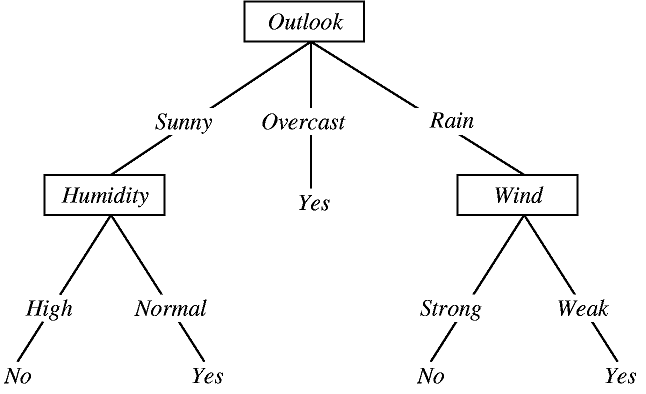
\includegraphics[width=0.4\linewidth]{figures/dt.png}
  \caption{An example of a decision tree.}
  \label{fig:dt}
\end{figure}
Decision trees (DTs) are decision support tools that use a tree-like model of decisions and their possible consequences,
including chance event outcomes, resource costs, and utility. In machine learning specifically, decision trees usually represent
a classification model where starting from a root node that contains the entirety of the dataset, and splitting based
on some criteria (gini index~\cite{gini} or entropy) we eventually arrive at leaves that contain sufficiently pure
subsets of the original dataset. Figure \ref{fig:dt} shows an example of a decision tree.

There are several ways to train a decision tree. Two of the most popular algorithms are CART~\cite{cart} and ID3~\cite{id3dt}.
Both methods use a splitting goodness criterion to divide the dataset into two partitions at each split in a greedy manner
that best improves the purity of the resultant nodes. It has been shown that constructing the optimal decision tree is NP-complete~\cite{dtnpcom}, 
hence why we have to resort to greedy approaches in order to feasibly construct decision trees.


\subsubsection{Random Forest}
An extension of DTs and a subset of ensemble machine learning models that aims to improve the generalization and stability of
a DT by generating a myriad of DTs, each trained on a subset of the dataset and on a subset of the available features and then
producing a final prediction by performing a majority voting on all of the trained DTs~\cite{randomforests}.

\subsubsection{k-NN}
Arguably one of the simplest classifiers available, k-NN\footnote{k-Nearest Neighbors} classifies any given data point on the basis
of its closeness to previously seen samples in a predefined neighborhood. More concretely, the $k$ closest samples to any given sample
are specified based on a distance metric (usually Minkowski distance of order 2, $d(p, q) = \|p-q\|$) and then the class of the sample
in question is determined by a majority voting from these $k$ samples. The main idea here is that if in a fixed neighborhood, a given sample
is closest to samples of some class $\omega$, then the sample itself probably also belongs to the same class.~\cite{knn}

Moreover, there is a trade-off between overfitting and underfitting w.r.t. the hyperparameters $k$. However, a statistical analysis at~\cite{kinknn}
shows that a generally good optimal value for $k$ is $\sqrt{N}$ where $N$ is the number of available samples. 

Although simple, the k-NN classifier has some strong consistency results. As the number of samples ($N$) approaches infinity,
the two-class k-NN is guaranteed to yield an error rate no worse than twice the Bayes optimal error rate.

For a general case Cover and Hart prove in~\cite{knnbounds} an upper bound error rate of
\begin{equation}
  R^* \le R_{kNN} \le R^*(2-\frac{MR^*}{M-1})
\end{equation}
where $R^*$ is the Bayes optimal error rate, $R_{kNN}$ is the error associated with k-NN classifier
and $M$ is the number of classes. For the two-class case, using (11) and as $R^*$ approaches 0, we have
\begin{equation}
  R^* \le R_{kNN} \le 2R^*
\end{equation}

\subsubsection{AdaBoost}
Originally conceived by Yoav Freund and Robert Schapire in 1995~\cite{adaboost}, AdaBoost is a statistical classification meta-algorithm 
that can be used in conjunction with many other types of learning algorithms to improve performance. The idea is to start from an ensemble of 
weak classifiers that perform marginally better than a random classifier. Then at every step, by increasing the weight of the misclassified samples
by this ensemble, we make the entirety of the classifier more robust to classification errors. 

More concretely, a boosted classifier is a classifier of the form
\begin{equation}
  F_T(x) = \sum_{t=1}^T f_t(x)
\end{equation}
where each $f_t$ is a weak learner that as input a vector $x$ and returns a value representing the class of that input vector.
At each iteration $t$, a weak learner is selected and assigned a weight $\alpha_t$ such that the total training
error $E_t$ of the resulting $t$-staged boosting classifier (in (14)) is minimized.
\begin{equation}
  E_t = \sum_i E[w_{i,t} F_{t-1}(x_i) + \alpha_t h(x_i)]
\end{equation}
Here $F_{t-1}(x)$ is the boosted classifier that has been built up to the previous stage of the training and
$f_t(x) = \alpha_t h(x)$ is a weak learner that is being considered for addition to the final ensemble of classifiers.
Moreover, at each iteration a weight $w_{i,t}$ is assigned to each sample in the training set equal to the current error $E(F_{t-1}(x_i))$ 
so that over time, the classifier becomes more robust to classification errors.
\subsubsection{MLP}
\begin{figure}
  \centering
  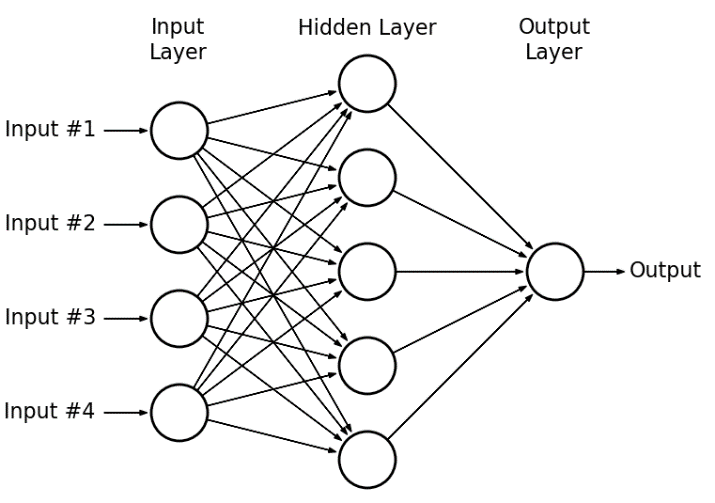
\includegraphics[width=0.4\linewidth]{figures/mlp.png}
  \caption{Structure of an MLP}
  \label{fig:mlp}
\end{figure}
Considered to be one of the oldest classification techniques, MLPs\footnote{Multi-Layer Perceptrons} are extremely strong classifiers that are
able to create non-convex decision surfaces and have the ability to approximate any function to an arbitrary precision. MLP is a fully connected class of
feedforward ANNs\footnote{Artificial Neural Networks}. Figure \ref{fig:mlp} shows the structure of 2-layer MLP. A matrix of weights is associated with each layer and the output of each layer $l$ is computed as
\begin{equation}
  \begin{gathered}
    a_l = f(n_l)\\
    n_l = w^T a_{l-1} + b_l
  \end{gathered}
\end{equation}
where $f(.)$ is a non-linear activation function (such as $tanh$, $relu$ or $sigmoid$). Through a process of back propagation, the weights
of this network are updated by means of SGD\footnote{Stochastic Gradient Descent} which, in essence, calculates the gradient of the cost function that penalizes the
network output by the amount it differs from the expected output, w.r.t. to each individual weight in each layer. This gradient is then deducted
from the weights of each of the parameters with the hopes of nudging the network in the direction of a minimum.

Due to the convergence stability issues of the initial versions of SGD, several improvements, including momentum SGD~\cite{sgdm} which is used here were proposed
that improve convergence speed and stability of the learning process.

\subsection{Experiment Setup}
The fabled Python machine learning suite, Scikit-learn~\cite{sklearn} was used in order to implement the classifiers described above.
The implementation python notebook file, `\text{methods\_comparison.ipynb}' is readily available and is accompanied by this article.

The hyperparameters with which each of the classifiers were deployed are as follows:
\begin{itemize}
  \item Logistic Regression: \begin{itemize}
    \item Regularization: $L2$ norm of weights added to the loss function
  \end{itemize}
  \item C-SVM: \begin{itemize}
    \item C: $1$
    \item Kernel: Linear
  \end{itemize}
  \item Naive Bayes: \begin{itemize}
    \item Variance Smoothing Epsilon Value: $10^{-9}$
  \end{itemize}
  \item Decision Tree: \begin{itemize}
    \item Splitting Criterion: Gini index
    \item Min. Samples to Split: $2$
    \item Min. Impurity Decrease: $0$
  \end{itemize}
  \item Random Forest: \begin{itemize}
    \item Decision Tree Properties: Same as above.
    \item Max. Number of Features Used for an Individual Tree: $\sqrt{N}$ where $N$ is the number of features.
    \item Number of Decision Trees Built: $100$
  \end{itemize}
  \item k-NN: \begin{itemize}
    \item Metric: Minkowski distance
    \item k: $\sqrt{N}$ where $N$ is the number of available samples.
  \end{itemize}
  \item AdaBoost: \begin{itemize}
    \item Number of Weak Learners: $200$
    \item Weight applied to each Weak Classifier at every Iteration (Learning Rate): 1
  \end{itemize}
  \item MLP: \begin{itemize}
    \item Two Hidden Layers with $100$ and $50$ neurons each to ensure non-convex decision surface.
    \item Activation of Hidden Layers: $relu$
    \item Last Layer Activation: $sigmoid$
    \item Optimizer: Variable Learning Rate Momentum SGD
    \item Initial Learning Rate: $0.0001$
    \item Momentum ($\gamma$): $0.9$
    \item Maximum Iterations: $2000$
  \end{itemize}
\end{itemize}

\section{Experiments and Results}
A global random state seed was set so that the experiments are repeatable with the same results presented in this paper.
Each of the classifiers discussed in previous sections was trained on the dataset in order to perform the binary classification task of voice gender recognition.
The experiments were run twice, once without and once with PCA to reduce the dimensionality of the feature space.
\subsection{Before PCA}
Before performing dimensionality reduction, the results of the experiments can be observed in figures \ref{fig:no_pca_comp} and \ref{fig:no_pca_cm}.
As we can see, Random Forest and AdaBoost have had the best performance on the dataset and Naive Bayes classifier is the worst by a notable margin.

Because Scikit-learn uses Decision Trees as the weak learners for its AdaBoost implementation, the mean accuracy achieved by Random Forest and AdaBoost
is similar, although as seen in the confusion matrices, the behavior of the two classifiers is not exactly the same.
\begin{figure}[h]
  \centering
  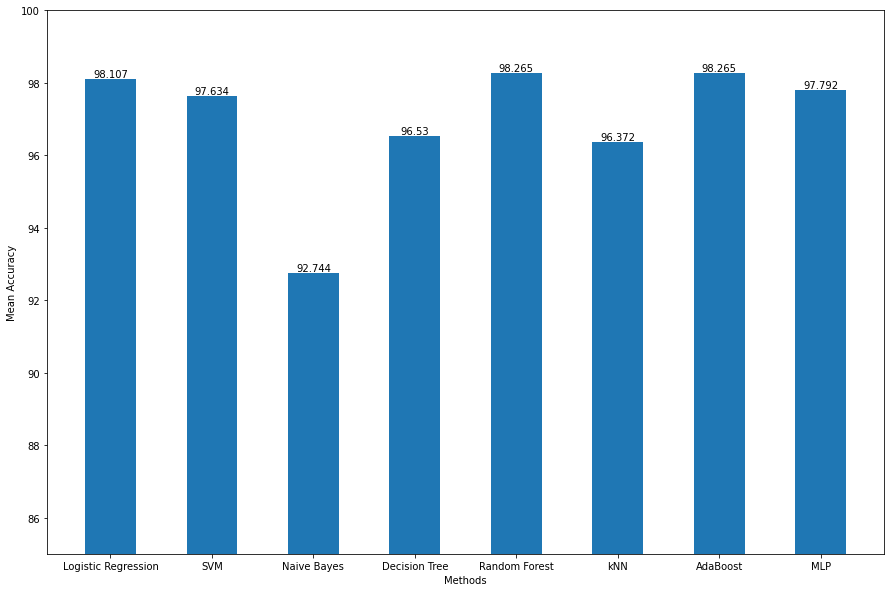
\includegraphics[width=0.95\linewidth]{figures/no_pca_comparison.png}
  \caption{Confusion Matrices of Each Classifier on the Dataset Before PCA}
  \label{fig:no_pca_comp}
\end{figure}
\begin{figure}[hbtp]
  \centering
  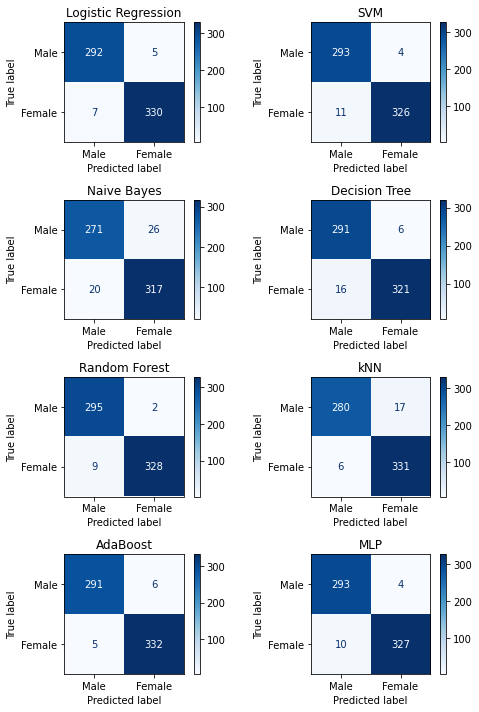
\includegraphics[width=0.8\linewidth]{figures/no_pca_conf_mats.png}
  \caption{Confusion Matrices of Each Classifier on the Dataset Before PCA}
  \label{fig:no_pca_cm}
\end{figure}
\clearpage
\subsection{After PCA}
Before we move on to the experiments, it is not without merit to take a look at the 
distribution of the classes over the two principal axes to see how separable they are
if we only chose to take the two components corresponding to the two biggest eigenvalues.
\begin{figure}[t]
  \centering
  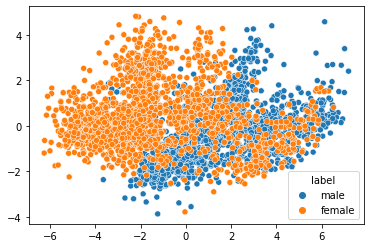
\includegraphics[width=0.6\linewidth]{figures/pca_visualization.png}
  \caption{visualization of the Dataset over the Two Principal Axes}
  \label{fig:pca_vis}
\end{figure}
As is evident in figure \ref{fig:pca_vis}, even the two most informative axes alone are already enough to give a reasonable representation
of the dataset. In our experiments however, we have use all the principal axes up to the point where 90\% of the information is preserved.
This results in a dimensionality reduction from the original $17$-d feature space, to only $8$ features, while still giving comparable results
to the experiments performed before PCA as we can see in figures \ref{fig:pca_comp} and \ref{fig:pca_cm}. 
\begin{figure}[h]
  \centering
  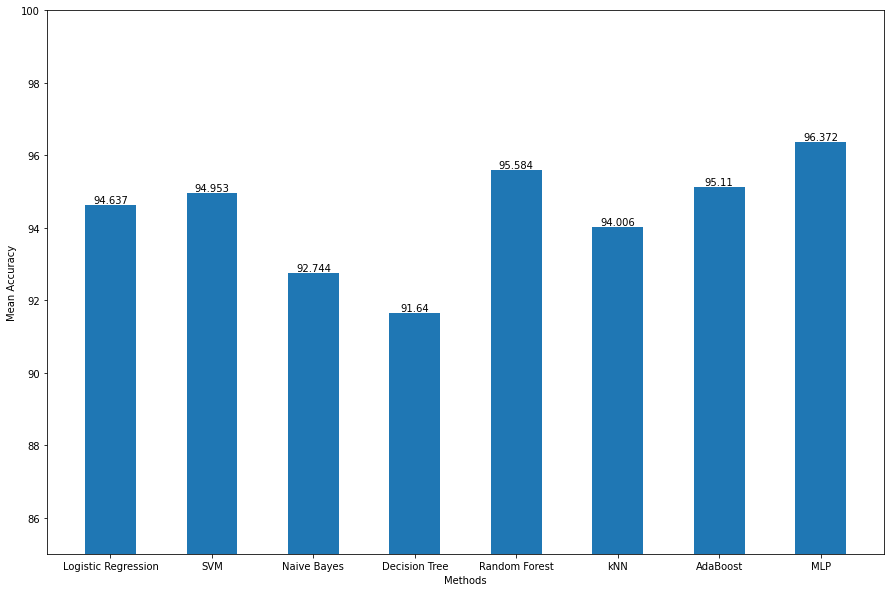
\includegraphics[width=0.95\linewidth]{figures/pca_comparison.png}
  \caption{Confusion Matrices of Each Classifier on the Dataset After PCA}
  \label{fig:pca_comp}
\end{figure}
\begin{figure}[hbtp]
  \centering
  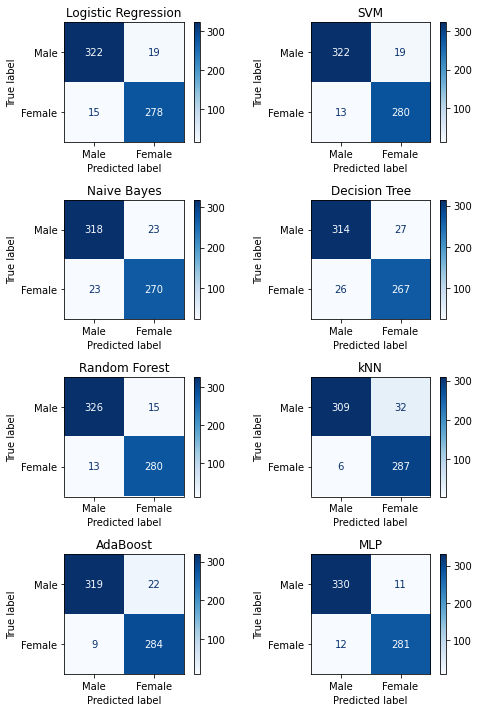
\includegraphics[width=0.8\linewidth]{figures/pca_conf_mats.png}
  \caption{Confusion Matrices of Each Classifier on the Dataset After PCA}
  \label{fig:pca_cm}
\end{figure}
\clearpage
We can see that in the reduced space, MLP performs the best followed by Random Forest, while
Decision Tree comes in last, even below Naive Bayes. Interestingly enough, the mean accuracy of 
the Naive Bayes classifier is affected the least by performing PCA on the dataset. Overall, an average of about \~3\% 
mean accuracy was lost going from the complete feature space to the reduced feature space which is negligible against
the gain obtained from reducing the feature space down to only 8 features.

It is also important to note that in both comparisons, Random Forest has performed strictly better than a single Decision Tree.


% needed in second column of first page if using \IEEEpubid
%\IEEEpubidadjcol


% An example of a floating figure using the graphicx package.
% Note that \label must occur AFTER (or within) \caption.
% For figures, \caption should occur after the \includegraphics.
% Note that IEEEtran v1.7 and later has special internal code that
% is designed to preserve the operation of \label within \caption
% even when the captionsoff option is in effect. However, because
% of issues like this, it may be the safest practice to put all your
% \label just after \caption rather than within \caption{}.
%
% Reminder: the "draftcls" or "draftclsnofoot", not "draft", class
% option should be used if it is desired that the figures are to be
% displayed while in draft mode.
%
%\begin{figure}[!t]
%\centering
%\includegraphics[width=2.5in]{myfigure}
% where an .eps filename suffix will be assumed under latex, 
% and a .pdf suffix will be assumed for pdflatex; or what has been declared
% via \DeclareGraphicsExtensions.
%\caption{Simulation results for the network.}
%\label{fig_sim}
%\end{figure}

% Note that the IEEE typically puts floats only at the top, even when this
% results in a large percentage of a column being occupied by floats.


% An example of a double column floating figure using two subfigures.
% (The subfig.sty package must be loaded for this to work.)
% The subfigure \label commands are set within each subfloat command,
% and the \label for the overall figure must come after \caption.
% \hfil is used as a separator to get equal spacing.
% Watch out that the combined width of all the subfigures on a 
% line do not exceed the text width or a line break will occur.
%
%\begin{figure*}[!t]
%\centering
%\subfloat[Case I]{\includegraphics[width=2.5in]{box}%
%\label{fig_first_case}}
%\hfil
%\subfloat[Case II]{\includegraphics[width=2.5in]{box}%
%\label{fig_second_case}}
%\caption{Simulation results for the network.}
%\label{fig_sim}
%\end{figure*}
%
% Note that often IEEE papers with subfigures do not employ subfigure
% captions (using the optional argument to \subfloat[]), but instead will
% reference/describe all of them (a), (b), etc., within the main caption.
% Be aware that for subfig.sty to generate the (a), (b), etc., subfigure
% labels, the optional argument to \subfloat must be present. If a
% subcaption is not desired, just leave its contents blank,
% e.g., \subfloat[].


% An example of a floating table. Note that, for IEEE style tables, the
% \caption command should come BEFORE the table and, given that table
% captions serve much like titles, are usually capitalized except for words
% such as a, an, and, as, at, but, by, for, in, nor, of, on, or, the, to
% and up, which are usually not capitalized unless they are the first or
% last word of the caption. Table text will default to \footnotesize as
% the IEEE normally uses this smaller font for tables.
% The \label must come after \caption as always.
%
%\begin{table}[!t]
%% increase table row spacing, adjust to taste
%\renewcommand{\arraystretch}{1.3}
% if using array.sty, it might be a good idea to tweak the value of
% \extrarowheight as needed to properly center the text within the cells
%\caption{An Example of a Table}
%\label{table_example}
%\centering
%% Some packages, such as MDW tools, offer better commands for making tables
%% than the plain LaTeX2e tabular which is used here.
%\begin{tabular}{|c||c|}
%\hline
%One & Two\\
%\hline
%Three & Four\\
%\hline
%\end{tabular}
%\end{table}


% Note that the IEEE does not put floats in the very first column
% - or typically anywhere on the first page for that matter. Also,
% in-text middle ("here") positioning is typically not used, but it
% is allowed and encouraged for Computer Society conferences (but
% not Computer Society journals). Most IEEE journals/conferences use
% top floats exclusively. 
% Note that, LaTeX2e, unlike IEEE journals/conferences, places
% footnotes above bottom floats. This can be corrected via the
% \fnbelowfloat command of the stfloats package.
\section{Conclusion}
In this study, we have compared the performance of eight different popular machine learning classification frameworks 
on a tabular dataset before and after dimensionality reduction. In addition to this comparison, we have also shown the powerful
effect that dimensionality reduction can have on some datasets where reducing the feature space to half can result in negligible losses
of accuracy. 

Overall, the more complex methods like AdaBoost, MLP and Random Forests seem to have had the best classification results over all.





% if have a single appendix:
%\appendix[Proof of the Zonklar Equations]
% or
%\appendix  % for no appendix heading
% do not use \section anymore after \appendix, only \section*
% is possibly needed

% use appendices with more than one appendix
% then use \section to start each appendix
% you must declare a \section before using any
% \subsection or using \label (\appendices by itself
% starts a section numbered zero.)
%

\clearpage
% use section* for acknowledgment
\section*{Acknowledgment}


The author would like to thank Dr. Mohammad Reza Ahmadzadeh for their invaluable guidance over the course of the semester.


% Can use something like this to put references on a page
% by themselves when using endfloat and the captionsoff option.
\ifCLASSOPTIONcaptionsoff
  \newpage
\fi



% trigger a \newpage just before the given reference
% number - used to balance the columns on the last page
% adjust value as needed - may need to be readjusted if
% the document is modified later
%\IEEEtriggeratref{8}
% The "triggered" command can be changed if desired:
%\IEEEtriggercmd{\enlargethispage{-5in}}

% references section

% can use a bibliography generated by BibTeX as a .bbl file
% BibTeX documentation can be easily obtained at:
% http://mirror.ctan.org/biblio/bibtex/contrib/doc/
% The IEEEtran BibTeX style support page is at:
% http://www.michaelshell.org/tex/ieeetran/bibtex/
\bibliographystyle{IEEEtran}
% argument is your BibTeX string definitions and bibliography database(s)
%\bibliography{IEEEabrv,../bib/paper}
%
% <OR> manually copy in the resultant .bbl file
% set second argument of \begin to the number of references
% (used to reserve space for the reference number labels box)
\bibliography{citations}
\end{document}